\section{Reconstrucción}

A la salida del bloque de detección de marcadores se tiene, para cada cámara y para cada cuadro de una secuencia adquirida, un conjunto de coordenadas en dos dimensiones $(x,y)$ que ubican la posición en la imagen de aquellos marcadores que fueron detectados.
El proceso de reconstrucción consiste en obtener las coordenadas en tres dimensiones de la posición de los marcadores en el espacio,  a partir de la posición de los marcadores en al menos dos retinas.
En la Figura \ref{fig: esquema_reconstruccion} se muestra un bosquejo de la reconstrucción de un marcador usando para esto la detección de marcadores en dos cámaras.\\

\begin{figure}[ht!]
\begin{center}
%\includegraphics[scale=0.20]{img/Reconstruccion/ejemplo_reconstruccion.png}
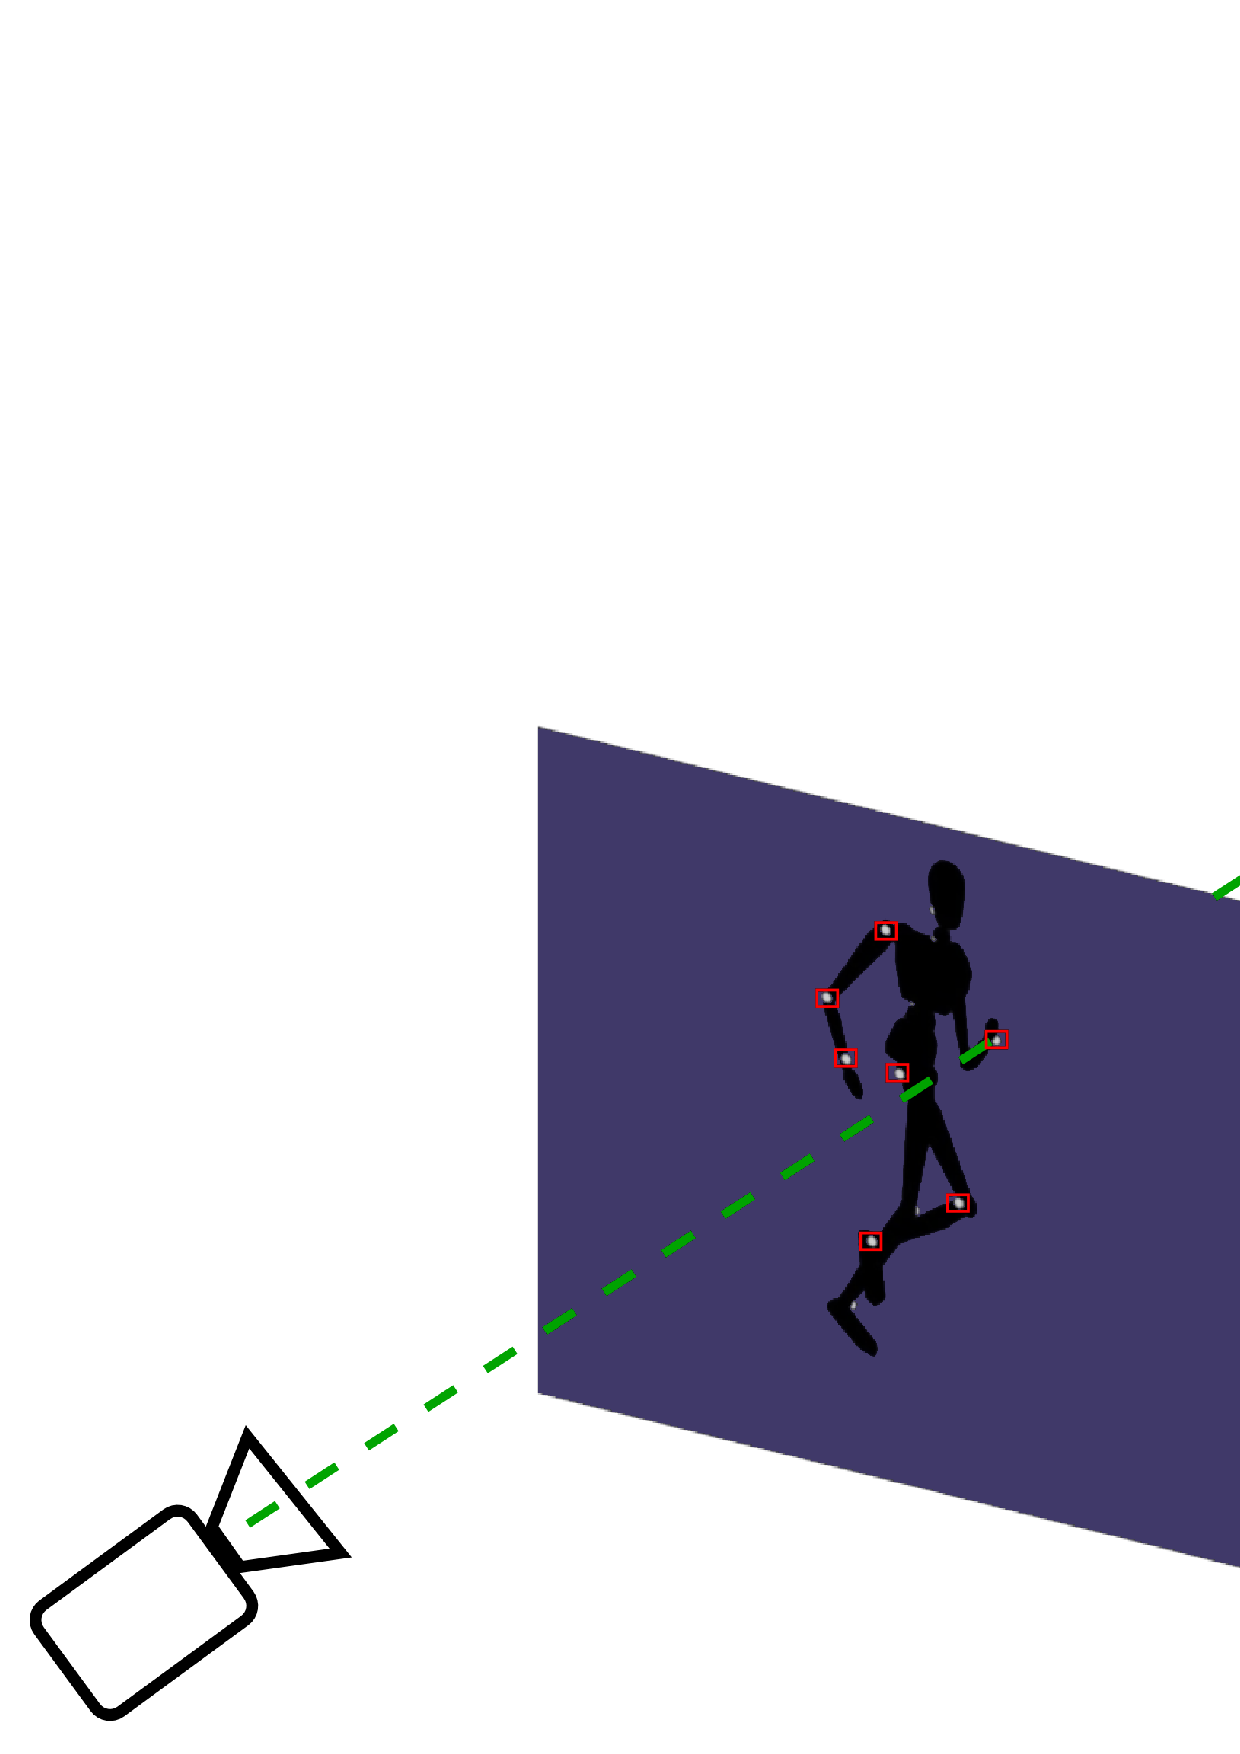
\includegraphics[scale=0.15]{../imagenes/Reconstruccion/reconstruccion.png}

\caption{Reconstrucción con dos cámaras.}
\label{fig: esquema_reconstruccion}
\end{center}
\end{figure}


El proceso de reconstrucción implementado fue inspirado en el trabajo de Herda \cite{herda} y consiste en tres pasos fundamentales:
\begin{enumerate}
\item Encontrar la correspondencia entre puntos en retinas diferentes.
\item Seleccionar la mejor correspondencia.
\item Reconstruir y verificar en el resto de las retinas.
\end{enumerate}

\subsection{Algoritmo}
El algoritmo implementado recibe como entrada los puntos 2D de los marcadores detectados y devuelve como salida los puntos 3D reconstruidos. El primer paso consiste en establecer una asociación entre ciertos puntos 2D de distintas cámaras. Luego, se pasa a un conjunto de bloques que se ejecutan de manera iterativa hasta que no queden marcadores para reconstruir. En dicho bloque se busca la mejor asociación entre puntos, bajo determinado criterio, luego se reconstruye un punto 3D y se realiza un proceso de validación de dicha reconstrucción. En la iteración siguiente se actualizan las asociaciones que habían sido establecidas previamente. Cuando no hay más marcadores para reconstruir se detiene el proceso iterativo y se devuelven aquellos marcadores que fueron reconstruidos en cada iteración. En la Figura \ref{fig: diagrama algoritmo} se presenta un diagrama del algoritmo.

\begin{figure}[ht!]
\begin{center}
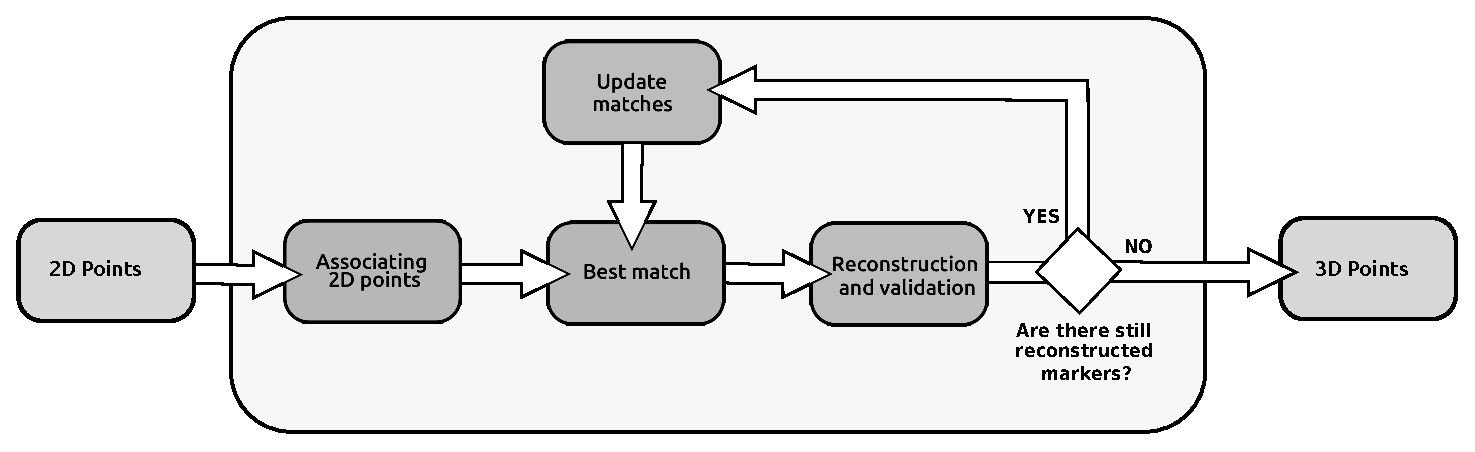
\includegraphics[scale=0.35]{../imagenes/Reconstruccion/bloques_reconstruccion}
\caption{Diagrama de bloques del algoritmo de reconstrucción.}
\label{fig: diagrama algoritmo}
\end{center}
\end{figure}

\subsubsection{Asociar puntos 2D}\label{seccion_asociar2D_uno}

Este bloque recibe como entrada las coordenadas de los puntos detectados en cada una de las cámaras, parámetros de las mismas tales como sus matrices de proyección y devuelve para cada punto una lista ordenada por relevancia, de las asociaciones existentes con puntos en otras cámaras.
Basándose en lo explicado anteriormente el proceso  se puede ejemplificar  en la Figura \ref{fig: cam2cam } y los pasos a seguir son los siguientes:

\begin{figure}[ht!]
\begin{center}
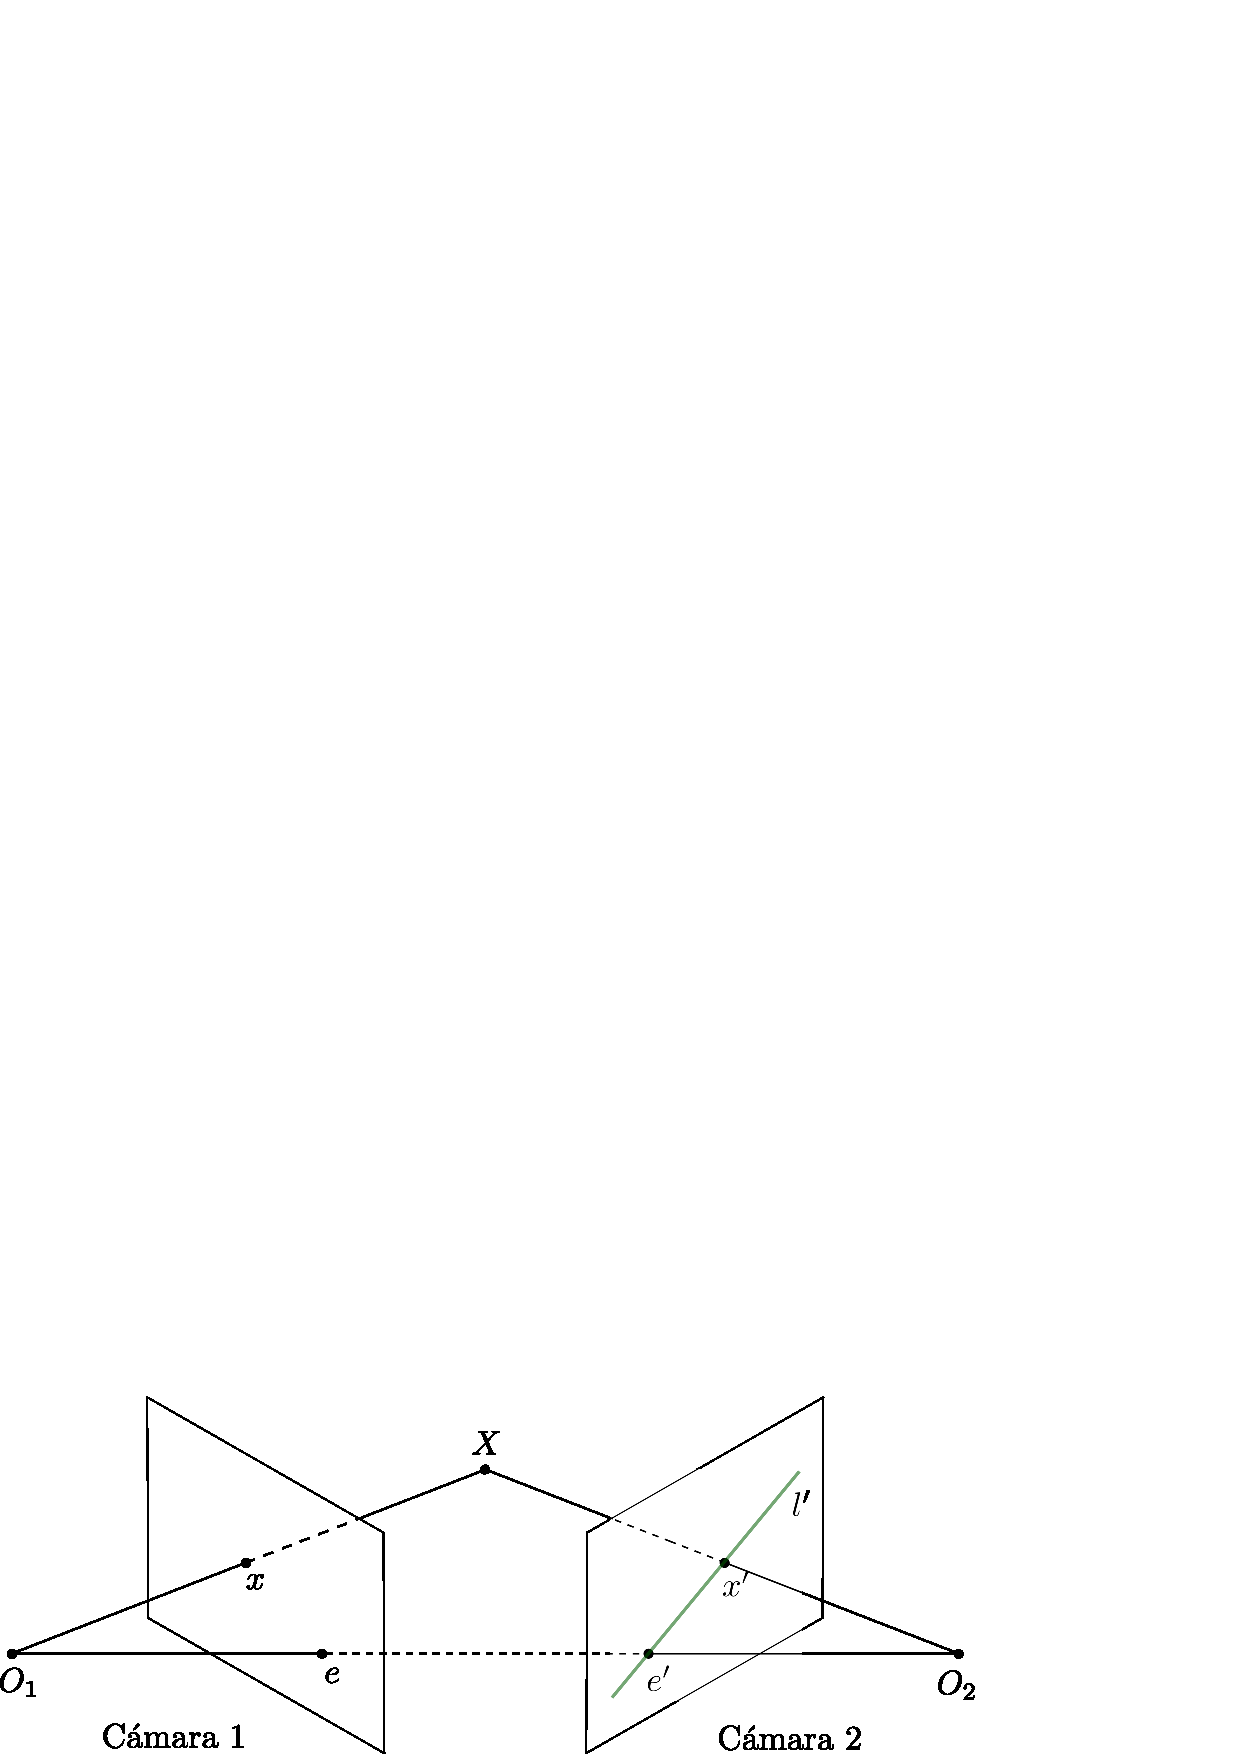
\includegraphics[scale=0.4]{../imagenes/Reconstruccion/geometria_epipolar.png}
\caption{Asociación de puntos 2D en dos cámaras.}
\label{fig: cam2cam }
\end{center}
\end{figure}

\begin{itemize}

\item Seleccionar dos cámaras y considerar un punto en una de ellas, por ejemplo el punto $x_{11}$ de la cámara 1.
\item Proyectar la recta epipolar $l_{11}$ correspondiente al punto $x_{11}$ sobre la cámara 2.
\item Tomar las distancias de los puntos detectados en la cámara 2 a la recta $l_{11}$.
\end{itemize}
Se asume que los puntos de la cámara 2 que tengan mayor posibilidad de corresponder con el punto $x_{11}$, son aquellos que al ser evaluados por la ecuación obtienen valores próximos a cero.
De esta manera se obtiene para cada punto en la cámara 1 un conjunto de puntos en la cámara 2 ordenados según su distancia a la recta epipolar correspondiente.
Repitiendo el procedimiento de manera inversa, esto es, de la cámara 2 a la cámara 1, se obtiene igualmente para cada punto de la cámara 2  los puntos de la cámara 1 ordenados según su proximidad a la recta epipolar correspondiente. A continuación se toman otros pares de cámaras y se vuelve a repetir el proceso. 

Es importante resaltar que para la elección de los pares de cámaras se han considerado dos casos.
El primero de ellos evalúa cada cámara respecto a todas las restantes y el segundo considera la disposición de las cámaras en el espacio y empareja las cámaras adyacentes de manera consecutiva.

EN CONSTRUCCIONNNNNNNNNNNNNN

esto es para probar las citas \cite{herda}

\subsubsection{Subsubsection Heading Here}
Subsubsection text here.
